\chapter{Package Contents \& Requirements}
\label{ch:package_contents}

Before you begin setting up the Mountain Climber Health \& GPS Tracker system, ensure that all components are present in your package and that you meet the necessary system requirements.

\section{What's in the Box}

The standard expedition kit includes the hardware items detailed in Table~\ref{tab:box_contents}. Carefully unpack all items and inspect them for any physical damage sustained during shipping.

\begin{table}[htbp]
    \centering
    \begin{tabular}{llc}
        \toprule
        \textbf{Item} & \textbf{Description} & \textbf{Quantity} \\
        \midrule
        Climber Main Device & Ruggedized ESP32 with GPS and LoRa modules & 1 \\
        Wristband & Wearable vitals monitor (ESP32, MAX30102) & 1 \\
        Repeater Unit & Range-extending LoRa relay node & 1 \\
        Base Camp Unit & Receiver node for connecting to the dashboard & 1 \\
        USB Cables & Micro-USB / USB-C cables for charging and data & 4 \\
        Mounting Straps & Velcro and elastic straps for securing devices & 1 set \\
        Quick Start Card & Basic pairing and SOS instructions & 1 \\
        \bottomrule
    \end{tabular}
    \caption{Standard Package Contents}
    \label{tab:box_contents}
\end{table}

\begin{figure}[H]
    \centering
    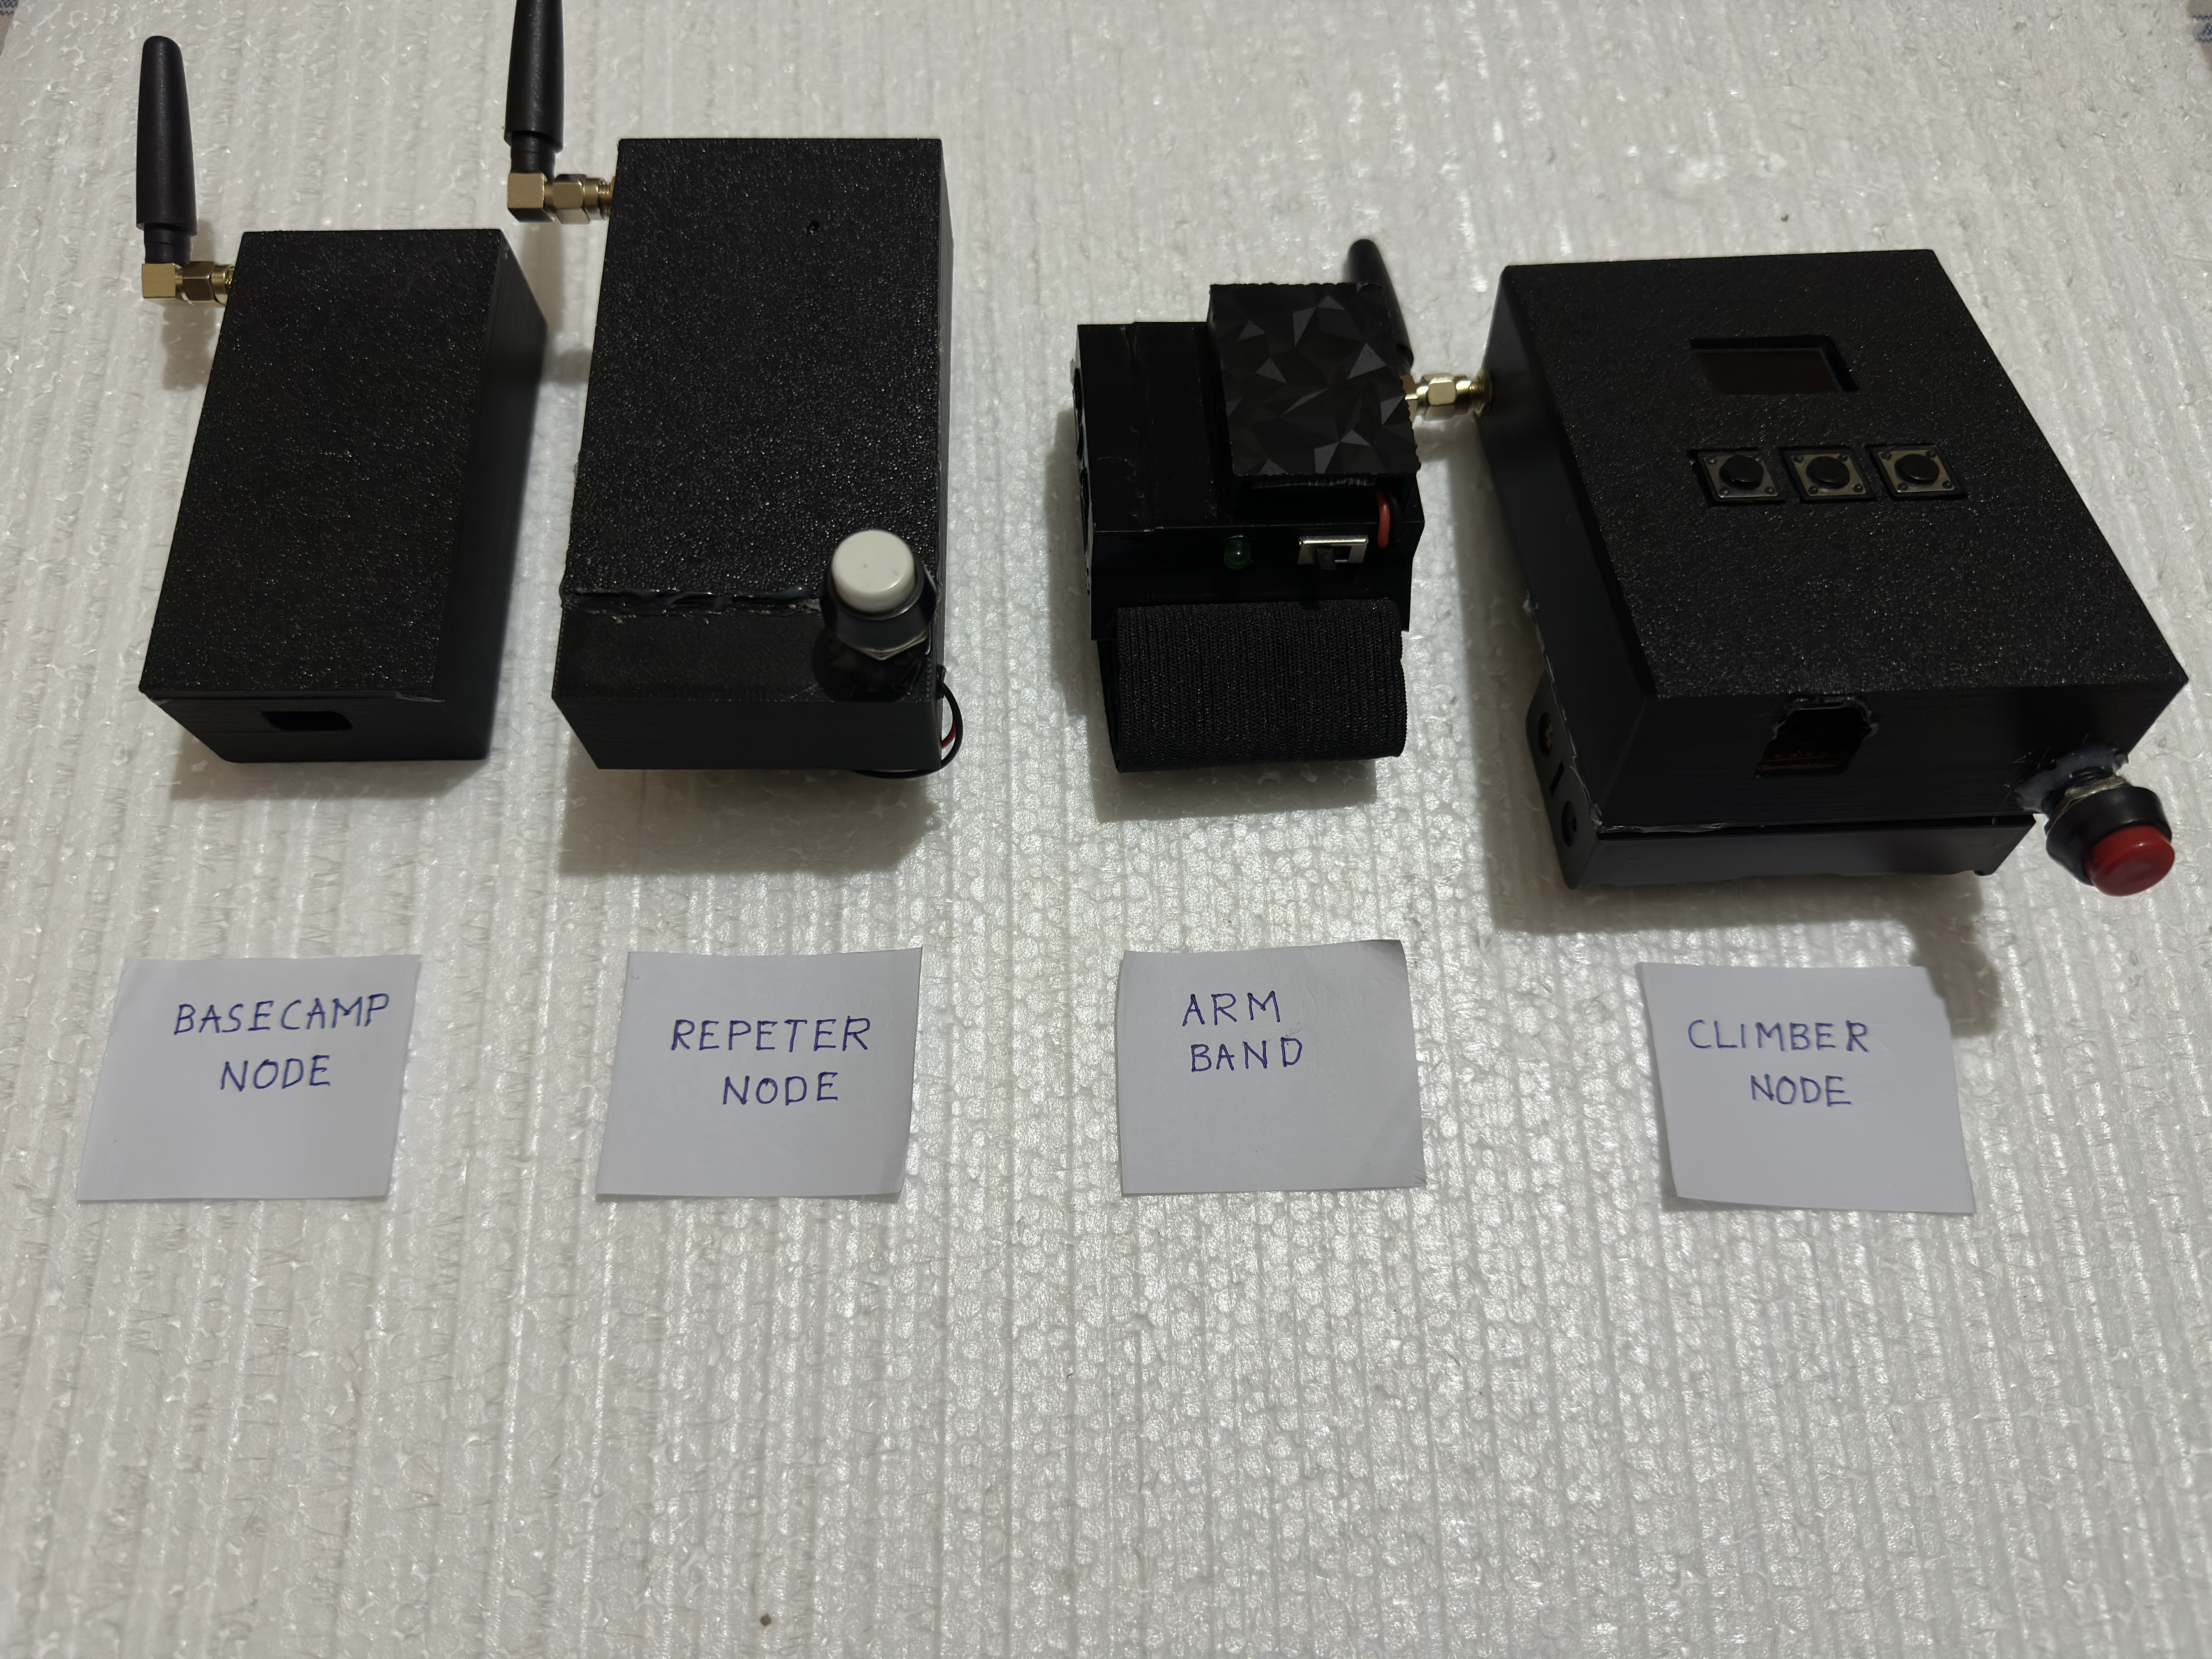
\includegraphics[width=0.8\textwidth]{figures/package_contents.png}
    \caption{Photo displaying all the unboxed contents of the Mountain Climber Tracker package.}
    \label{fig:package_contents}
\end{figure}

\section{System Requirements and Prerequisites}

To successfully deploy and operate the system, the following external equipment and capabilities are required:

\subsection{For the Climber}
\begin{itemize}
    \item \textbf{Smartphone:} An Android or iOS smartphone with Bluetooth 4.0 (BLE) support.
    \item \textbf{Mobile App:} The official Mountain Climber Tracker app installed (downloadable via the Web Portal or relevant App Stores).
    \item \textbf{Power Bank (Optional but Recommended):} For extended expeditions to recharge the Climber Main Device or Phone.
\end{itemize}

\subsection{For the Base Camp Operator}
\begin{itemize}
    \item \textbf{Laptop/Computer:} A reliable laptop running Windows, macOS, or Linux.
    \item \textbf{USB Port:} At least one available USB Type-A or Type-C port for connecting the Base Camp Unit.
    \item \textbf{Dashboard Software:} The Python Flask Dashboard application (provided as a standalone executable via PyInstaller) installed on the laptop.
    \item \textbf{WiFi Capability:} To connect to the Base Camp Unit's SoftAP network, if wireless monitoring is preferred over the USB serial connection.
\end{itemize}

\begin{infobox}
Internet access at the base camp is \textbf{not} required for real-time monitoring and SOS handling, as the LoRa mesh and Dashboard run completely locally. However, internet is required if you wish to sync logged data to the centralized Supabase portal post-expedition.
\end{infobox}
